\section{Question 2}
Satellite position and velocity vectors in the Earth-Centered Inertial (ECI) coordinate system:
$$
\vec{r}_{ECI} = \begin{bmatrix}-346 & 8265 & 4680\end{bmatrix}_{\textrm{km}}^{\textrm{T}}
$$

$$
\vec{v}_{ECI} = \begin{bmatrix}-5.657 & -1.73 & 2.703\end{bmatrix}_{\textrm{km}/\sec}^{\textrm{T}}
$$


\subsection{part a}
Algorithm for converting from ECI to  orbital x-y plane coordinates is described below:
\begin{enumerate}
\item Calculate the angular momentum vector $\vec{h}$ by taking the cross product of the position vector $\vec{r}$ and the velocity vector $\vec{v}$ in the ECI coordinate system.
\item Calculate the unit vector $\hat{z}$ in the direction of $\vec{h}$.
\item Calculate the unit vector $\hat{x}$ in the x-direction of the satellite position.
\item Calculate the unit vector $\hat{y}$ in the y-direction of the orbital plane by taking the cross product of $\hat{z}$ and $\hat{x}$.
\item Express the ECI position and velocity vectors $\vec{r}$ and $\vec{v}$ in the new coordinate system by taking their dot products with $\hat{x}$, $\hat{y}$, and $\hat{z}$.
\item Project the position and velocity vectors onto the x-y plane by setting the z-component of each vector to zero.
\end{enumerate}

Note: Above algorithm is implemented in the jupyter notebook file Q2.ipynb.

results:

$$
r_{\textrm{x, y plane}} \begin{bmatrix}
    9504.3327488 & 0 & 0
\end{bmatrix}_{\textrm{km}}^{\textrm{T}}
$$
$$
\vec{v}_{\textrm{x, y plane}} \begin{bmatrix}
    0 & 4.16567802 & 0
    \end{bmatrix}_{\textrm{km}/\sec}^{\textrm{T}}
$$

\subsection{part b}
To calculate satellite position after 30 minutes, the differential equation for the satellite solved for 30 minutes. The differential equation is:
$$
\vec{r}_{\textrm{x, y plane}} = \vec{v}
$$
$$
\frac{d\vec{v}}{dt} = -\frac{\mu}{r^3}\vec{r}
$$
where $\mu$ is the gravitational parameter of the Earth, and $r$ is the magnitude of the position vector $\vec{r}$.
Note: Above algorithm is implemented in the jupyter notebook file Q2.ipynb.

results:
$$
\vec{r}_{\textrm{x, y plane}} = \begin{bmatrix}
    1379.53 & 4493.87 & 0
\end{bmatrix}_{\textrm{km}}^{\textrm{T}}
$$
$$
\vec{v}_{\textrm{x, y plane}} = \begin{bmatrix}
    -9.72 -2.96 & 0
    \end{bmatrix}_{\textrm{km}/\sec}^{\textrm{T}}
$$

\begin{figure}[H]
    \centering
    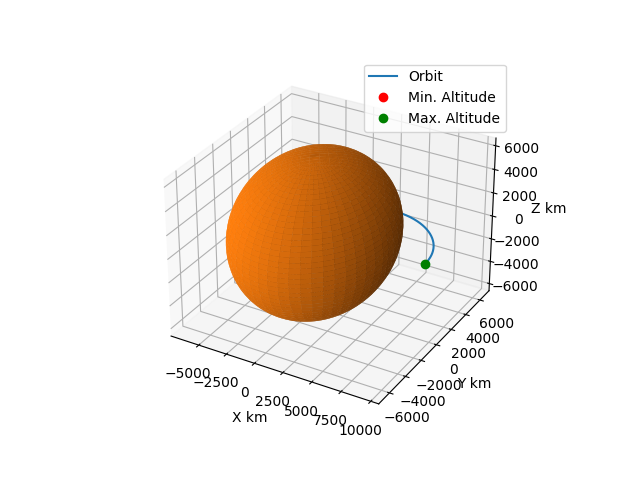
\includegraphics[width=\textwidth]{../Figure/Q2/satellite_orbit.png}
    \caption{The position of the spacecraft in the GCRF coordinate system.}
    \label{fig:fig1}
\end{figure}